\documentclass[tikz]{standalone}
\usepackage{tikz,amsmath}
\usetikzlibrary{shapes}
\begin{document}
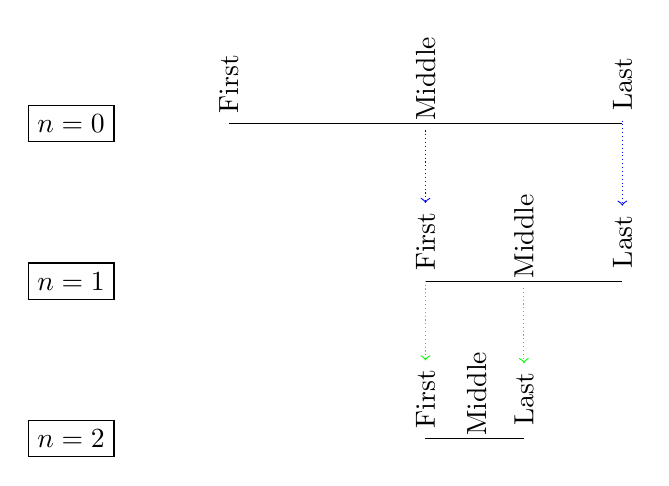
\begin{tikzpicture}

    \draw [-] (0,1) -- (5,1);
    \node [rectangle, draw] at (-2,1) {$n=0$};
    \node [rectangle, rotate=90] at (0,1.5) {First};
    \node (a)[rectangle, rotate=90] at (5,1.5) {Last};
    \node (A)[rectangle, rotate=90, xshift=2] at (2.5,1.5) {Middle};

    \draw [-] (2.5,-1) -- (5,-1);
    \node [rectangle, draw] at (-2,-1) {$n=1$};
    \node (b) [rectangle,  rotate=90] at (2.5,-.5) {First};
    \node (B) [rectangle,  rotate=90] at (5,-.5) {Last};
    \node (B') [rectangle,  rotate=90, xshift=2] at (3.75,-.5) {Middle};

    \draw [-] (2.5,-3) -- (3.75,-3);
    \node [rectangle, draw] at (-2,-3) {$n=2$};
    \node (c) [rectangle,  rotate=90] at (2.5,-2.5) {First};
    \node (C) [rectangle,  rotate=90] at (3.75,-2.5) {Last};
    \node [rectangle,  rotate=90, xshift=2] at (3.15,-2.5) {Middle};

    \draw [densely dotted, ->, color=blue] (a) -- (B);
    \draw [densely dotted, color=blue, ->] (A) -- (b);
    \draw [densely dotted, color=green, ->] (B') -- (C);
    \draw [densely dotted, color=green, ->] (b) -- (c);
%
%    \node [rectangle, draw] at (4,3) {14};
%    \node [rectangle, draw] at (4,2.5) {15};
%    \draw [color=red] (3.75,3.25) -- (4.25,2.25);
%    \draw [color=red] (3.75,2.25) -- (4.25,3.25);
%
%    \node [rectangle, draw] at (4,0) {23};
%    \node [rectangle, draw] at (4,-.5) {52};
%    \node [rectangle, draw] at (4,-1) {73};
%
%    \draw [->] (4.5,-.5) -- (5.5,1);
%    \draw [->] (4.5,-.5) -- (5.5,-1.75);
%
%    \node [rectangle, draw] at (6,1) {23};
%
%    \node [rectangle, draw] at (6,-1.5) {52};
%    \node [rectangle, draw] at (6,-2) {73};
%    \draw [color=red] (5.75,-1.25) -- (6.25,-2.25);
%    \draw [color=red] (5.75,-2.25) -- (6.25,-1.25);
%
%    \draw [->] (6.5,1) -- (7.5,1);
%
%    \node [rectangle, draw] at (8,1) {23};
%    \draw [color=red] (8,1) circle (.5);
\end{tikzpicture}
\end{document}
